\section{More Name Binding Patterns}
\appendixlabel{more-coverage}

In this appendix we discuss more name binding patterns and their encoding using
scope graphs.

\subsection{Definition-before-use}

\begin{wrapfigure}[13]{r}{0.51\textwidth}
\vspace*{-1\baselineskip}
\begin{boxedminipage}{\hsize}
\centering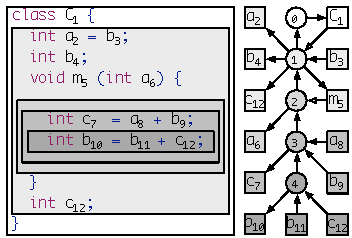
\includegraphics{figures/scope-graphs/subsequent/vars.pdf}
\end{boxedminipage}
\vspace*{-\baselineskip}
\caption{Subsequent scoping of Java variables modeled by nested scopes.}
\figurelabel{java:vars}
\end{wrapfigure}

Our scopes are sets of mutually recursive declarations. This makes it easy to
model a construct such as \pcfmcode{letrec} as we have seen in \Section{coverage}.
However, the scope constructs in many languages have a `definition before use'
policy in which bindings are only visible to references appearing `later' in the
program.
% (\TODO{speculate on the origin of such policies; Such a policy is a natural
% result of one-pass compilers.}) 
For example, the variable declarations in a
block in C or Java are only visible to the subsequent statements in the block.
While colloquially such a block is thought of as a single scope, in fact each
variable declaration opens a new scope, much like the bindings in the sequential
let construct.
\Figure{java:vars} shows how the policy is encoded for blocks in Java by placing
each declaration in a new scope that dominates the references in subsequent
statements.

% For example, in ML, the declaration of a variable with a def \TODO{notation?} is
% only visible \emph{after} in the remainder of the scope in which it is declared

%\paragraph{subsequent scope}
%
% notes about name binding rules in Java (?)
%
% The scope of a formal parameter of a method, constructor, or lambda expression is 
%   the entire body of the method, constructor, or lambda expression.
% 
% The scope of a local variable declaration in a block is the rest of the block in which the declaration appears, 
%   starting with its own initializer and including any further declarators to the right in the local variable declaration statement.
% 
% The scope of a local variable declared in the ForInit part of a basic for statement 
%   includes all of the following:
%   Its own initializer
%   Any further declarators to the right in the ForInit part of the for statement
%   The Expression and ForUpdate parts of the for statement
%  The contained Statement
% 
% The scope of a local variable declared in the FormalParameter part of an enhanced for statement is 
%   the contained Statement.
% 
% A declaration $d$ of a local variable named $n$ shadows, throughout the scope of $d$, 
%   the declarations of any other fields named $n$ that are in scope at the point where $d$ occurs, and 
%   the declarations of any other variables named $n$ that are in scope at the point where $d$ occurs but are not declared in the innermost class in which $d$ is declared.
% 
% It is a compile-time error if the name of a formal parameter is used to 
%   declare a new variable within the body of the method, constructor, or lambda expression, 
%   unless the new variable is declared within a class declaration contained by the method, constructor, or lambda expression.
% 
% It is a compile-time error if the name of a local variable $v$ is used to 
%   declare a new variable within the scope of v, 
%   unless the new variable is declared within a class whose declaration is within the scope of $v$.




% \paragraph{Field Access Modifiers in Java.}
% 
% \TODO{Don't understand this paragraph at all, really.}
% The previous example is imprecise, since it does not consider field access modifiers.
% This keeps \javacode{private} and \javacode{protected} fields visible,
%   yielding additional resolutions.
% From an IDE perspective, these resolutions are valuable, since they hint to
%   possible resolutions, when access modifiers are changed.
% Erroneous resolutions to \javacode{private} fields can be filtered by a language-specific well-formedness predicate,
%   which rejects resolution paths using imports of class scopes.
% Erroneous resolutions to \javacode{protected} requires a more sophisticated well-formedness predicate,
%   which considers the package scope of both class declarations. 

% The scope of a declaration of a member $m$ declared in or inherited by a class
% type $C$ is the entire body of $C$, including any nested type declarations.
% 
% A declaration $d$ of a field named $n$ shadows, throughout the scope of $d$, the
% declarations of any other variables named $n$ that are in scope at the point
% where $d$ occurs.

\subsection{Compilation Units and Packages in Java}

Scopes do not always correspond to single, continuous program fragments.
For example, in Java~\cite{JLS8}, 
  the scope of a top-level type name is all type declarations in the package in which it is declared.
Those type declarations can be spread over multiple, discontinuous program fragments,
  since a package can consist of a number of compilation units.

A compilation unit can be modeled as a scope,
  which imports other scopes associated with the same package name.
For example, 
  \Figure{java:units} shows two compilation units contributing to the same package \javacode{p}.
Each compilation unit declares package \javacode{p} in the root scope
  and associates the declaration with a scope for top-level type declarations.
Types \javacode{C} and \javacode{D} are declared in separate scopes, 
  but are reachable in both scopes via imports from scopes associated with \javacode{p}.
This approach follows the Java terminology, where each compilation unit declares its package.

\begin{figure}[t]
\begin{minipage}{0.42\textwidth}
\begin{boxedminipage}{\hsize}
\centering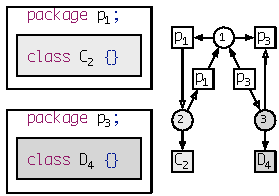
\includegraphics{figures/scope-graphs/java/units.pdf}
\end{boxedminipage}
\caption{Java compilation units modeled by import edges.}
\figurelabel{java:units}
\end{minipage}
\hfill
\begin{minipage}{0.56\textwidth}
\begin{boxedminipage}{\hsize}
\centering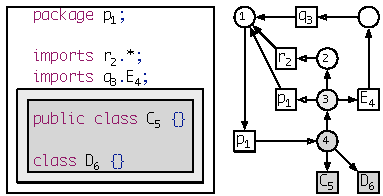
\includegraphics{figures/scope-graphs/java/imports.pdf}
\end{boxedminipage}
\caption{Java import declarations modeled by nested lexical scopes.}
\figurelabel{java:imports}
\end{minipage}
\end{figure}

\paragraph{Import Declarations.}

\Figure{java:imports} shows a compilation unit with two import declarations.
Java supports two kinds of type-import declarations in compilation units.
A \emph{single-type-import declaration} 
  imports a single type.
A \emph{type-import-on-demand declaration} 
  allows all accessible types of a package or type to be imported as needed. 
Thereby, types imported by single-import declarations shadow 
  types of the same name imported by import-on-demand declarations, 
  as well as top-level types of the same name declared in other compilation units of the same package.
The scope of an imported type name is all type declarations in the compilation unit in which the import declaration appears.

We model visibility of imported declarations by three lexical scopes per compilation unit.
The first scope handles all import-on-demand declarations.
The second scope 
  imports type declarations from other compilation units of the same package,
  and declares aliases for single-type-import declarations.
Those aliases act as a declaration and as a reference to the imported name.
According to the default visibility policy, 
  the alias declarations shadow imported declarations from the second and first scopes.
The third scope is associated with the package name and 
  declares the types of the compilation unit.
Those local declarations shadow declarations from other compilation units or packages.

\paragraph{Example.}

The scope graph diagram in \Figure{java:imports} shows 
  a root scope for package names and three lexical scopes for the compilation unit.
Scope $2$ imports from a package \javacode{r}
  and scope $3$ imports from other compilation units from package \javacode{p}.
The single-import declaration \javacode{q.E} is modeled as a qualified name resolution in the global scope
  and as a declaration in scope $3$.
Scope $4$ declares the top-level types \javacode{C} and \javacode{D}.

\paragraph{Accessibility.}

In Java, the reachability of type declarations can be influenced by access modifiers.
In the example, \javacode{C} and \javacode{D} can be accessed in other compilation units of \javacode{p},
  but \javacode{D} cannot be accessed in other packages.
To model accessibility, we need to distinguish 
  \javacode{public}  from \emph{package-private} classes, and
  imports of compilation units of the same package from regular imports in the scope graph.
We can then define a Java-specific well-formedness predicate which rejects
  paths with regular imports of package-private classes.

\subsection{Namespaces and Partial Classes in C\#}

While Java packages can be declared in multiple compilation units,
  C\# namespaces are open-ended,
  allowing also for multiple declarations of a namespace in the same compilation unit.
In a similar way, C\# supports open-ended class declarations.
\Figure{csharp:partial} shows two declarations of namespace \javacode{N}, 
  both partially declaring a class \javacode{C}.
The left part declares a field \javacode{f},
  while the right part is referring to this field.
Similar to Java import declarations, 
  the using directive in the left part only affects the left namespace declaration. 
  
We can model those partial scopes similarly to packages in Java.
Each namespace declaration corresponds to two lexical scopes,
  where local declarations in the second scope hide imported declarations in the first scope.
The second scope also imports from other namespace declarations for the same namespace.
The same pattern can be applied for partial class declarations.
However, C\# supports proper nesting of namespaces and partially qualified names.
Thus, we can no longer resolve to other partial declarations of the same name in global scope.
With the default reachability policy,
  we might find other partial declarations for the same name in lexical scope.
Instead, we need to make sure to resolve only to parts in the same surrounding namespace 
  (which might again be declared in several parts).
This can be achieved by distinguishing imports of parts from regular imports,
  and a reachability policy for the former, which rejects parent paths. 

\begin{figure}[t]
\begin{boxedminipage}{\hsize}
\centering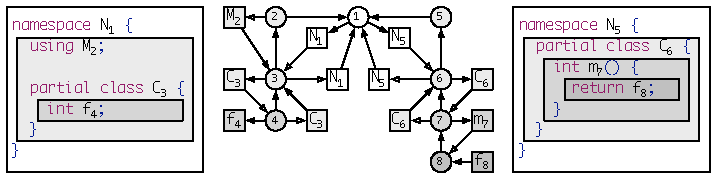
\includegraphics{figures/scope-graphs/csharp/partial.pdf}
\end{boxedminipage}
\caption{C\# namespaces and partial classes modeled by import edges.}
\figurelabel{csharp:partial}
\end{figure}

%%%%%%%%%%%%%%%%%%%%%%%%%%%%%%%%%%%%%%%%%%%%%%%%%%%%%%%%%
\endinput
  %\usepackage{graphics} is needed for \includegraphics
\begin{figure}[h]
\begin{minipage}{3cm}
\begin{lstlisting}[language=Java]
val x = 1;
{ 
  import p.x;
  x // ambiguous reference
}
\end{lstlisting}
\end{minipage}
  \caption{Java package and type declarations in different compilation units.}
  \label{figureLabel}
\end{figure}





%\subsection{PCFM}
	  
		systematic discussion of typical examples and corner cases
		
		collect all the examples in this section 
		
		
%\subsection{Namespaces.}

Some programming languages distinghuish different kinds of names. A reference of
one kind cannot refer to a declaration of another kind of name.
For example, in Java, classes, class variables, and methods are distinct kinds
of names, which do not interfere.
In ML, variables and algebraic datatype constructors are distinguished
syntactically by requiring that constructors start with a capital and variables
with a lower case letter. 
In the NaBL name binding DSL this notion is
characterized using the concept of \emph{namespaces} \cite{KonatKWV12}.

In this paper, we do not explicitly consider the notion of namespaces,
effectively assuming a single namespace.
However, this is not a limitation, since namespaces can be encoded by mapping a
name in a program to a pair of its namespace and the name. For example, we can
distinghuish a variable with name $x$ from a method with name $x$ by encoding
them as $(V, x)$ and $(M, x)$, respectively.
\GW{
  It is a limitation for references, since it requires to know the namespace before resolution. 
  Java's ambiguous names cannot be modeled this way.
}
\GW{
  Obscuring is another interesting topic here. Can we handle this by (language-specific) disambiguation?
  \emph{
    A simple name may occur in contexts where it may potentially be interpreted as the name of a variable, a type, or a package. 
    In these situations, the rules of §6.5 specify that a variable will be chosen in preference to a type, and that a type will be chosen in preference to a package. 
    Thus, it is may sometimes be impossible to refer to a visible type or package declaration via its simple name.
  }
}
\EV{Perhaps this discussion is somewhat distracting and not relevant for the
flow of the story at this position anyway and could be moved to a later point in
the paper, such as the extensions section 4.}

%\subsection{Multiple source files.}

Programs are typically distributed over multiple source files and name binding
crosses file boundaries.
Scopes do not need to correspond to nodes in an
AST, but can represent virtual code units such as a project or library.
The scope graphs for the ASTs of the individual files are joined under a common
scope.
